\section{Best practices}
\label{talloc:sec:best-practices}

The following sections contain several best practices and good manners that were
found by the Samba and SSSD developers during the years. Those will help you to
write a better code, easier to debug and with as little (hopefully none) memory
leaks as possible.

\subsection{Keep the context hierarchy steady}

The talloc is a hierarchy memory allocator. The hierarchy nature is what makes
the programming more error proof. It makes the memory easier to manage and free.
Therefore the first thing we should have on our mind is: always project our data
structures into the talloc context hierarchy.

That means if we have a structure, we should always use it as a parent context
for its elements. This way we will not encounter any troubles when freeing this
structure or when changing its parent. The same rule applies for arrays.

For example, the structure |user| which is defined in the Listing
\ref{struct-user} (page \pageref{struct-user}) should be created with the
context hierarchy illustrated in Figure \ref{fig:bp-context-tree}.

\begin{figure}[H]
  \centering
  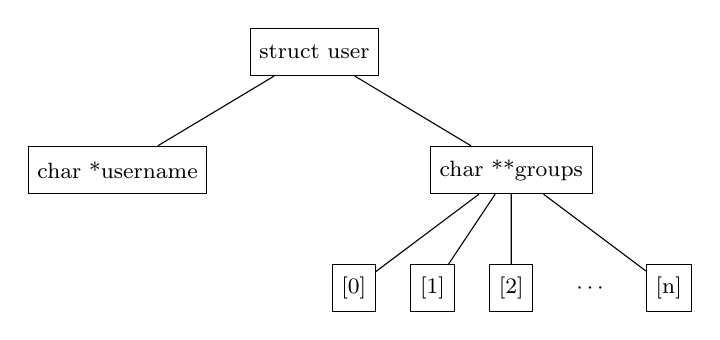
\begin{tikzpicture}
[level/.style={sibling distance=10mm},
 level 1/.style={sibling distance=50mm},
 every node/.style=
   {minimum height=6mm,rectangle,draw=black,font=\footnotesize}]
\node [] {struct user}
  child {node [] {char *username} }
  child {node [] {char **groups}
    child {node [] {[0]}}
    child {node [] {[1]}}
    child {node [] {[2]}}
    child {node [draw=none] {$\cdots$} edge from parent[draw=none]}
    child {node [] {[n]}}
  };
\end{tikzpicture}
  \caption{Context tree of struct user}
  \label{fig:bp-context-tree}
\end{figure}

\subsection{Every function should use its own context}
\label{talloc:subsec:function-use-own-context}

It is a good practice to create a temporary talloc context at the function
beginning and free this context just before the return statement. All the data
must be allocated on this context or on its children. This ensures that no
memory leaks are created as long as we do not forget to free the temporary
context.

This pattern applies to both situations - when a function does not return any
dynamically allocated value and when it does. However it needs a little
extension for the latter case.

\subsubsection{Functions that does not return any dynamically allocated value}

If the function does not return any value created on the heap, we will just obey
the aforementioned pattern.

\begin{lstlisting}[caption={Temporary context \#1},label=lst:tmp-ctx-1]
int bar()
{
  int ret;
  TALLOC_CTX *tmp_ctx = talloc_new(NULL);
  if (tmp_ctx == NULL) {
    ret = ENOMEM;
    goto done;
  }
  /* allocate data on tmp_ctx or on its descendants */
  ret = EOK;
done:
  talloc_free(tmp_ctx);
  return ret;
}
\end{lstlisting}

\subsubsection{Functions returning dynamically allocated values}

If our function returns any dynamically allocated data, its first parameter
should always be the destination talloc context. This context will serve
as a parent for the output values. But again, we will create the output values
as the descendants of the temporary context. If everything goes well, we will
change the parent of the output values from the temporary to the destination
talloc context.

This pattern ensures that if some error occurs (e.g. insufficient amount of
memory), all allocated data are freed and no garbage appears on the destination
context.

\begin{lstlisting}[caption={Temporary context \#2},label=lst:tmp-ctx-2]
int struct_foo_init(TALLOC_CTX *mem_ctx, struct foo **_foo)
{
  int ret;
  struct foo *foo = NULL;
  TALLOC_CTX *tmp_ctx = talloc_new(NULL);
  if (tmp_ctx == NULL) {
    ret = ENOMEM;
    goto done;
  }
  foo = talloc_zero(tmp_ctx, struct foo);
  /* ... */
  *_foo = talloc_steal(mem_ctx, foo);
  ret = EOK;
done:
  talloc_free(tmp_ctx);
  return ret;
}
\end{lstlisting}

\subsection{Allocate temporary contexts on NULL}
\label{talloc:subsec:tmp-ctx-on-null}

As you can see on the Listing \ref{lst:tmp-ctx-2}, instead of allocating the
temporary context directly on |mem_ctx|, we created a new top level context
using |NULL| as the parameter for |talloc_new()| function. Take a look at the
following example.

\begin{lstlisting}[caption={Temporary context \#3},label=lst:tmp-ctx-3]
char * create_user_filter(TALLOC_CTX *mem_ctx,
                          uid_t uid, const char *username)
{
  char *filter = NULL;
  char *sanitized_username = NULL;
  /* tmp_ctx is a child of mem_ctx */
  TALLOC_CTX *tmp_ctx = talloc_new(mem_ctx);
  if (tmp_ctx == NULL) {
    return NULL;
  }
  
  sanitized_username = sanitize_string(tmp_ctx, username);
  if (sanitized_username == NULL) {
    talloc_free(tmp_ctx);
    return NULL;
  }
  
  filter = talloc_aprintf(tmp_ctx,"(|(uid=%llu)(uname=%s))",
                          uid, sanitized_username);
  if (filter == NULL) {
    return NULL; /* tmp_ctx is not freed */ (*@\label{lst:tmp-ctx-3:leak}@*)
  }
  
  /* filter becomes a child of mem_ctx */
  filter = talloc_steal(mem_ctx, filter);
  talloc_free(tmp_ctx);
  return filter;
}
\end{lstlisting}

We forgot to free |tmp_ctx| before the |return| statement on line
\ref{lst:tmp-ctx-3:leak}. However it is created as a child of |mem_ctx| context
and as such it will be freed as soon as the |mem_ctx| is freed. Therefore no
detectable memory leak is created.

On the other hand we do not have any way how to access the allocated data
and for what we know |mem_ctx| may exists for a lifetime of our application.
For these reasons this should be considered as a memory leak. But how can we
detect it when it is properly freed? The only way is to notice the mistake in
the source code.

But if we create the temporary context as a top level context, it will not be
freed and memory diagnostic tools
(e.g. |valgrind|\footnote{\url{http://valgrind.org}}) are able to do their job.

\subsection{Temporary contexts and talloc pool}
\label{talloc:subsec:tmp-ctx-and-pool}

If we want to take the advantage of the talloc pool but also keep to the
pattern introduced in previous section, we are unable to do it directly. The
best thing to do is to create a conditional build where we can decide how do we
want to create the temporary context. For example, we can create following
macros:

\begin{lstlisting}[caption={Conditional temporary context
macros},label=lst:tmp-ctx-4]
#ifdef USE_POOL_CONTEXT
  #define CREATE_POOL_CTX(ctx, size) talloc_pool(ctx, size)
  #define CREATE_TMP_CTX(ctx)        talloc_new(ctx)
#else
  #define CREATE_POOL_CTX(ctx, size) talloc_new(ctx)
  #define CREATE_TMP_CTX(ctx)        talloc_new(NULL)
#endif
\end{lstlisting}

Now if our application is under development, we will build it with macro
|USE_POOL_CONTEXT| undefined. This way, we  can use memory diagnostic
utilities to detect memory leaks.

The release version will be compiled with the macro defined. This will  enable
pool contexts and therefore reduce the |malloc()| calls, which will end up in a
little bit faster processing.

\begin{lstlisting}[caption={Conditional temporary context},label=lst:tmp-ctx-5]
int struct_foo_init(TALLOC_CTX *mem_ctx, struct foo **_foo)
{
  int ret;
  struct foo *foo = NULL;
  TALLOC_CTX *tmp_ctx = CREATE_TMP_CTX(mem_ctx);

  ...
}

errno_t handle_request(TALLOC_CTX mem_ctx)
{
  int ret;
  struct foo *foo = NULL;
  TALLOC_CTX *pool_ctx = CREATE_POOL_CTX(NULL, 1024);
  
  ret = struct_foo_init(mem_ctx, &foo);
  ...
}
\end{lstlisting}